\chapter{Introduction}

This dissertation introduces a new approach to discovering context for photo annotation problems. The primary complexity of photo annotation problems lies in large search spaces of the solution and the diversity of feature-based representations of images. Contextual information is used to prune this large search spaces with reduced dependency on image features. Once the search space has been reduced, the image features are used to select from the \textit{remaining} tags. For example, people with weak social ties do not co-occur often in photos, and by identifying one we can eliminate the other. In this case, we would say that social context is used to prune candidates in a face annotation problem.

Recently, there have been two changes in the scientific community which motivates us to take a fresh look at context. First, with mobile phones becoming the primary mode of photo taking, the nature of context has evolved from providing cues about tags, to the description of the world around a photo taking moment when a person was taking the photo. With the ever increasing amount of personal, social and public information, it is becoming harder to specify which subset of these would constitute the most interesting context for a given picture. Thus, it is not clear what data to consider context, and how do we combine them to form models of the real world which will allow photo annotation algorithms to reason what tags to assign various regions in a given photo.

This dissertation addresses the problem of constructing computational representations of real world events from various heterogeneous data sources, to reason which parts of the search space can be pruned without hurting the overall performance of the annotation algorithm. We refer to such a representation as the \textbf{Context Network} of the photo. The network describes real-world events occurring in the environment, the entities participating in them, and their semantic inter-relationships.

\begin{figure}[t]
\centering
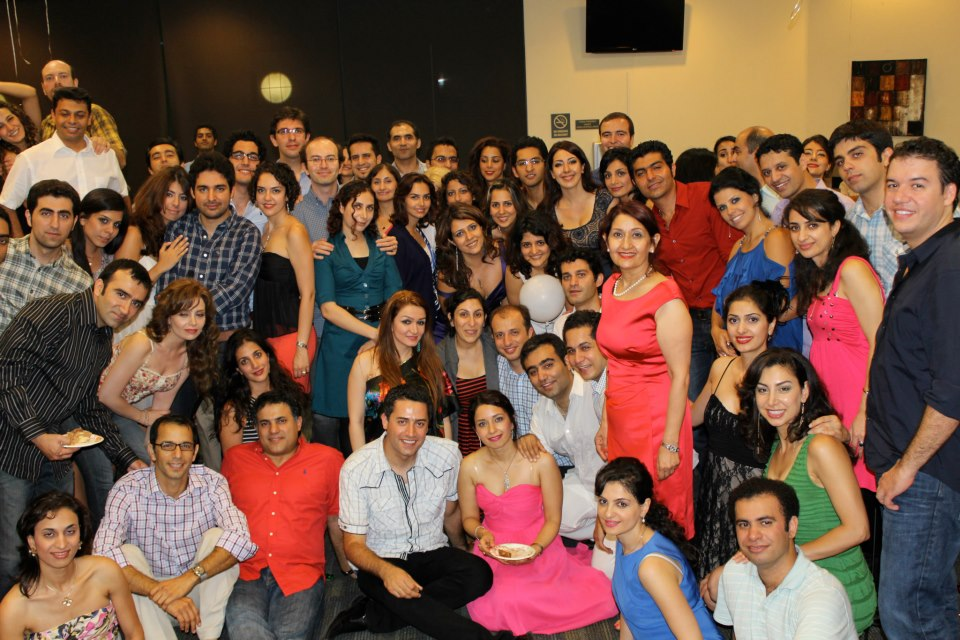
\includegraphics[width=0.8\textwidth]{media/chapter1/setarehetal}
\caption{Face tagging problems could be challenged by very large search spaces.}
\label{fig:people}
\end{figure}


\section{Importance}

Technique is applicable to a variety of problems which needs to reason about real world events.

\begin{figure}[t]
\centering
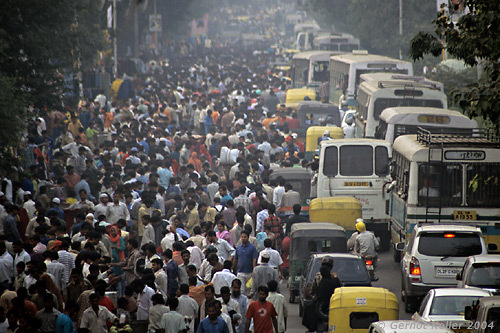
\includegraphics[width=0.75\textwidth]{media/chapter1/india-streets.jpg}
\caption{Such streets would pose a significant challenge in designing automomous cars.}
\label{fig:india-streets}
\end{figure}


\section{Novelty}

\section{Approach}
Before embarking on a mission to model the entire world, we ask ourselves the question: How much of the real world information is actually relevant to the intelligent system? Constructing the entire world model is extremely challenging and often unnecessary. For example, there might not be much value in representing sports events in New York in a model being used to help cars navigate in Japan. 

This primary \uline{contribution} of this dissertation is a \textbf{\textit{progressive discovery}} algorithm to ingest information from various real world data sources to construct context networks containing the most relevant information for pruning the search space for the system. Examples of data sources include social media web services to provide information about events and entities like Facebook, Twitter; services which can be queried to find information about places like Yelp; Sensors on personal mobile phones, for example GPS which inform applications of the location of a person is present at any given point in time.

\textbf{What is progressive discovery?} Progressive discovery is an incremental process where knowledge of real world events and entities can be added to a given context network. Given a context network and multiple data sources describing events and entities, a progressive discovery algorithm will obtain new information from the sources and relate it to context network. By iteratively executing this algorithm, we can grow a context network until the data sources can provide no further information or the information in the network prunes the search space well enough for the AI problem to be fully solved.

The discussion in the following chapters on context networks and their discovery from various data sources will be presented in conjunction with an application to \textbf{tag faces in personal photos}. The face tagging algorithm, whose search space contains a few million entities is a very hard real world AI problem. But if a real world model of the world existed, the search space which is relevant to this photo contains just the entities who are present within the field of view of the camera at the time the photo was captured. 

\section{Overview}
This dissertation is organized into the following chapters. Chapter 2 provides an overview of context, how context has been used to address problems in various scientific disciplines and how we use context in our specific personal photo tagging application. Chapter 3 describes the related work in computer science, and how this work is informed by them. Chapter 4 describes our context discovery framework, how it models various data sources, and how our progressive discovery algorithm constructs models for real world problems. We facilitate this discussion with an example real world application to tag faces of people in personal photos. Chapter 5 analyzes the algorithmic complexity of different parts of the system, and provides experiments to verify the competence and performance of the system. We also present experiments to confirm the efficacy of our approach in the light of the real world application. Finally, chapter 6 attempts to describe the future possibilities of using context discovery in computer science.

% Chapters 6 and 7 describe two extensions to the CueNet framework to solve problems of missing context and that of source selection. 

\section{Terminology}
Before starting the discussion on Context Networks, it is necessary to include a short note on terminology to avoid any ambiguities. We use the word `Object' to collectively refer to events and entities. An entity includes persons, places in the world, for example `Starbucks, UC Irvine', `The Eiffel Tower, Paris, France', or organizations, for example `Google Inc', `Royal Society of London'. The term `object' has been used in literature to refer to things which have no temporal properties. But, in our discussion, an `object' could imply an event which exhibits temporal properties.

\begin{figure}[h]
\centering
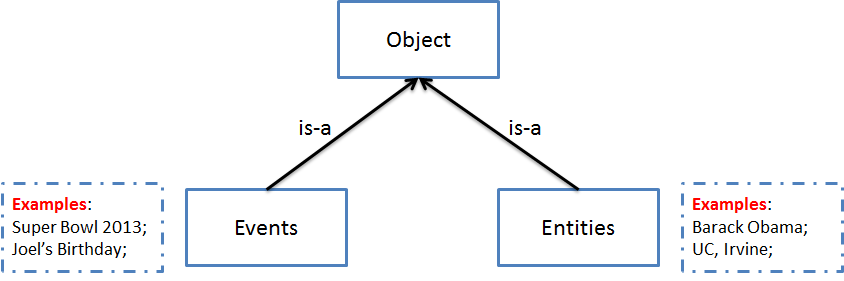
\includegraphics[width=0.75\textwidth]{media/chapter1/terminology.png}
\caption{Objects, Events and Entities.}
\label{fig:terminology}
\end{figure}
